\documentclass[conference]{IEEEtran}
\pdfoutput=1    % For arXiv issues


% -------------------------- COLORBLIND COLORS -------------------------------
% Use color palettes for colorblind people from
% https://davidmathlogic.com/colorblind/#%23D81B60-%231E88E5-%23FFC107-%23004D40 or https://colorbrewer2.org/
\usepackage{xcolor}
\definecolor{wong-black}        {HTML}{000000}
\definecolor{wong-lightorange}  {HTML}{E69F00}
\definecolor{wong-lightblue}    {HTML}{56B4E9}
\definecolor{wong-green}        {HTML}{009E73}
\definecolor{wong-yellow}       {HTML}{F0E442}
\definecolor{wong-darkblue}     {HTML}{0072B2}
\definecolor{wong-darkorange}   {HTML}{D55E00}
\definecolor{wong-pink}         {HTML}{CC79A7}

% -------------------------- PACKAGES -------------------------------

\usepackage{url}
\def\UrlBreaks{\do\/\do-}   % Line breaks of long URLs in biblatex bibliography (https://tex.stackexchange.com/questions/134191/line-breaks-of-long-urls-in-biblatex-bibliography)

\usepackage{hyperref} % Working hyperlink (https://www.overleaf.com/learn/latex/Hyperlinks)
\hypersetup{
    colorlinks=true,
    citecolor=wong-green,
    linkcolor=wong-darkblue,
    filecolor=wong-pink,      
    urlcolor=wong-black,
    pdfpagemode=FullScreen,
    }

% Use these to always use Fig. and Sec. instead of worrying about Figure, Fig, Fig. etc in the document
\newcommand{\figref}[1]{Fig.~\ref{#1}}
\newcommand{\secref}[1]{Sec.~\ref{#1}}

\usepackage{cite}
\usepackage{tabularx}
\usepackage{booktabs}
\usepackage{amsmath,amssymb,amsfonts}
\usepackage{algorithmic}
\usepackage{graphicx}
\usepackage{textcomp}
\usepackage[nolist, nohyperlinks, printonlyused]{acronym} % For consistent acronyms

\def\BibTeX{{\rm B\kern-.05em{\sc i\kern-.025em b}\kern-.08em
    T\kern-.1667em\lower.7ex\hbox{E}\kern-.125emX}}

%% orcid logo
\usepackage{scalerel}
\usepackage{tikz}
\usetikzlibrary{svg.path}


\definecolor{orcidlogocol}{HTML}{A6CE39}
\tikzset{
	orcidlogo/.pic={
		\fill[orcidlogocol] svg{M256,128c0,70.7-57.3,128-128,128C57.3,256,0,198.7,0,128C0,57.3,57.3,0,128,0C198.7,0,256,57.3,256,128z};
		\fill[white] svg{M86.3,186.2H70.9V79.1h15.4v48.4V186.2z}
		svg{M108.9,79.1h41.6c39.6,0,57,28.3,57,53.6c0,27.5-21.5,53.6-56.8,53.6h-41.8V79.1z M124.3,172.4h24.5c34.9,0,42.9-26.5,42.9-39.7c0-21.5-13.7-39.7-43.7-39.7h-23.7V172.4z}
		svg{M88.7,56.8c0,5.5-4.5,10.1-10.1,10.1c-5.6,0-10.1-4.6-10.1-10.1c0-5.6,4.5-10.1,10.1-10.1C84.2,46.7,88.7,51.3,88.7,56.8z};
	}
}

\newcommand\orcidicon[1]{\href{https://orcid.org/#1}{\mbox{\scalerel*{
				
\begin{tikzpicture}[yscale=-1,transform shape]
					\pic{orcidlogo};
				\end{tikzpicture}
			}{|}}}}
    
\newcommand\nnfootnote[1]{  % Footnote without hyperref association (https://tex.stackexchange.com/questions/415625/avoiding-hyperref-warning-ignoring-empty-anchor)
  \begin{NoHyper}
  \renewcommand\thefootnote{}\footnote{#1}%
  \addtocounter{footnote}{-1}%
  \end{NoHyper}
}

\begin{document}

% -------------------------- TITLE -------------------------------

\title{Definition of Test Oracles for Identifying TP, FP, and FN in Object Perception for Automated Driving}

%\title{Relevant Criteria for Identifying TP, FP, and FN in Dependability Assessment of Object Perception}


%\title{A Language to Specify a Test Oracle that Identifies TP, FP, and FN}


%\title{A Model to Define TP, FP, and FN for Dependable Object Perception}

% \title{A Model to Define True Positives, False Positives, and False Negatives for Dependable Object Perception}

% -------------------------- AUTHORS -------------------------------

\author{\IEEEauthorblockN{
		Michael Hoss$^{1} \orcidicon{0000-0001-9924-7596}$
	}

% \IEEEauthorblockA{\IEEEauthorrefmark{2}}
% \IEEEauthorblockA{\IEEEauthorrefmark{3}}
}

\maketitle

\nnfootnote{$^{1}$~The author is with RWTH Aachen University, Germany. {\tt\small \href{mailto:michael.hoss@rwth-aachen.de}{michael.hoss@rwth-aachen.de}}. 
\newline
Despite being the only author, the first person plural (``we") is used to comply with a common style of scientific writing. 
}

%\nnfootnote{\textasteriskcentered~These authors contributed equally}

% -------------------------- ACRONYMS -------------------------------

\begin{acronym}
    \acro{ml}[ML]{Machine Learning}
	\acro{cnn}[CNN]{Convolutional Neural Network}
	\acro{dl}[DL]{Deep Learning}
	\acro{ad}[AD]{Autonomous Driving}
\end{acronym}

% -------------------------- ABSTRACT -------------------------------


\begin{abstract}
%%Single paragraph up to 250 words. Mini-version of the paper that includes context, state of the art, why it is not good enough, the research question, the methods, the evaluation and conclusions.
Contemporary test methods for the perception subsystem of automated vehicles require a characterization of true-positive, false-positive, and false-negative object tracks. % general term for TP, FP, FN
The literature defines these concepts in various different ways, which impedes comparability across different works. 
To overcome this issue, this paper provides an exhaustive model to define these concepts as formally as possible.
The model generally describes the criteria for association of tracks under test to reference tracks. 
Emphasized details are object distance functions in state space including penalties and thresholds, multi-object association algorithms, reference data and labeling characteristics, geometric issues like fields of view and semantic areas, temporal issues like incomplete tracks, and generalizations to probabilistic world models and asynchronous time stamps. 
While a majority of aspects can be formalized, a case study illustrates the remaining challenges towards an entirely formal description. 





% Yannick feedback:
% - be more precise, more clear, and more confident in abstract
% - probably use a more standardized templated abstract strcture
% - maybe even put in abstract that I want to bring together the perception community and the v&v community


%Single paragraph up to 250 words. Mini-version of the paper that includes context, state of the art, why it is not good enough, the research question, the methods, the evaluation and conclusions.
Test methods for the perception subsystem of driving automation systems commonly identify true-positive (TP), false-positive (FP), and false-negative (FN) objects. % general term for TP, FP, FN
To date, these terms may be understood differently in different testing activities.
However, clear definitions are needed for their comparability and for a potential usage within a safety case. 
Therefore, this paper provides a set of relevant criteria for identifying TP, FP, and FN objects. % in an ideally unambiguous way.
% The criteria generally cover 
%that cover the generation of reference objects and their association to objects under test. 
Emphasized details are the level of the tested objects (e.g. detections or tracks), reference sensor characteristics, labeling policies, object distance functions, % in state space including penalties and thresholds, 
multi-object association, fields of view, areas of importance, incomplete tracks, asynchronous time stamps, and probabilistic object representations. 
% While a majority of aspects can be formalized, a case study illustrates the remaining challenges towards an entirely formal description. 
We find it challenging to characterize all aspects relevant for identifying TP, FP, and FN through adequate formal criteria due to both the open context problem and the symbol grounding problem.
Nevertheless, we encourage practitioners to define these aspects in their publications as formally as feasible. 
Uncertainties in these definitions likely remain and should therefore be accounted for in the induction of safety claims from statistics of TP, FP, and FN. 

\end{abstract}

% -------------------------- KEYWORDS -------------------------------

% \begin{IEEEkeywords}
% testing, environment perception, automated vehicles
% % component, formatting, style, styling, insert
% \end{IEEEkeywords}

% -------------------------- CONTENT -------------------------------


\section{Introduction}
\label{sec:introduction}

\subsection{Motivation}

The task of object-based environment perception for automated driving systems (ADS) receives much focus through public perception challenges. % that benchmark different approaches.
They publish datasets of raw sensor data along with reference labels for training purposes. 
Their leaderboards then rank individual submissions according to their similarity to the non-public reference labels on the test part of the dataset.

Common metrics of such leaderboards consist of aggregations of true-positive objects (TPs), false-positive objects (FPs), and false-negative objects (FNs). 
These direct metrics from the perception domain are comprehensible, straightforward to compute, and highly popular, but not necessarily adapted to the driving task. 
For example, it is typically unclear which FPs or FNs also lead to vehicle-level failures. 
% Assuming that every FP and FN leads to a vehicle-level failure would render the achievement of 
%Assuming that every FP or FN leads to a vehicle-level failure would be a tremendous overestimation that would 

To reduce and forecast vehicle-level failures, the field of safety assurance for automated driving has gained much popularity. 
One method of achieving provable safety is to decompose the driving automation system into different subsystems and establish dependable interfaces between them. 
The perception subsystem can be defined to consist of sensor hardware and computation for world modeling, excluding any prediction or planning into the future. 
Its dependability requires a sufficiently low mean time between events that induce vehicle-level failures. 
%Demonstrating this dependability is an active research questions that this paper aims to contribute to. 

% Or at least estimate how the perception outputs differ from the ground truth to construct sensor models for simulation tests.

The demonstration of this dependability is an active topic of research, where one of the most crucial issues is the identification of perception outputs that are not safe for the driving task. 
Task-oriented and safety-relevant perception metrics are therefore currently being proposed. 
In contrast to the most popular perception leaderboard metrics, safety-oriented metrics tend to be more complex and incomprehensible due to their additional consideration of the downstream driving function and of safety in road traffic. 
%Popularity of direct metrics that are based on TP, FP, FN still orders of magnitude higher than the popularity of task-oriented metrics. 

Ideally, novel perception metrics combine all desired properties such that they are helpful to both perception developers and verification and validation engineers. 
This requires closing the gap between straightforward safety-agnostic metrics and highly complex safety-relevant metrics. 
%comprehensible to humans, and straightforward to compute all at the same time. 

\subsection{Contributions}
While one could make safety-relevant metrics less complex, the present paper aims at making straightforward metrics better usable for safety assurance. 
Specifically, we aim at defining TPs, FPs, and FNs clearly enough such that statistics of them represent meaningful evidences for safety claims. 
%Differentiation between metric types:
%In contrast, downstream metrics from the safety domain are adapted to the driving task, but more difficult to understand, more difficult to compute, and still not as well researched. 
%These metrics, however, directly detect and penalize failures relevant to the driving task. 
%Consequently, we consider it worth while investigating whether metrics can be both easy to compute \textit{and} sufficient for safety claims.
%Context of this contribution:
%This paper provides potential tools for the definition of further perception metrics that are ideally task-oriented, safety-oriented, and easy to understand and compute. 
%Specifically, we aim at defining popular aspects of direct metrics clearly enough such that they can represent meaningful evidences for safety-relevant claims.  
Our main contributions are:
\begin{itemize}
\item A set of criteria to define how a test oracle identifies TPs, FPs, and FNs (Sec. \ref{sec:criteria})
\item A discussion of the relevance of TPs, FPs, and FNs in the safety assurance context (Sec. \ref{sec:discussion})
\end{itemize}


%This paper aims at contributing basic understanding of relevant at the intersection of perception and safety assurance. 


%Within the challenge to define useful safety-relevant perception metrics, this paper aims at 

%Can popular metrics based on TP, FP, and FN be adapted towards meaningful contributions within a safety case? 




The discussion will treat the following research questions:
\begin{itemize}


\item {RQ1}: \textit{Can TP, FP, and FN be objectively defined?}

\item {RQ2}: \textit{How relevant are TP, FP, and FN for task-oriented perception metrics?}

\item {RQ3}: \textit{Can statistics of TP, FP, and FN contribute to a safety argumentation?}
\end{itemize}

\begin{figure*}[t]
	\centering
	\vspace*{2mm}
	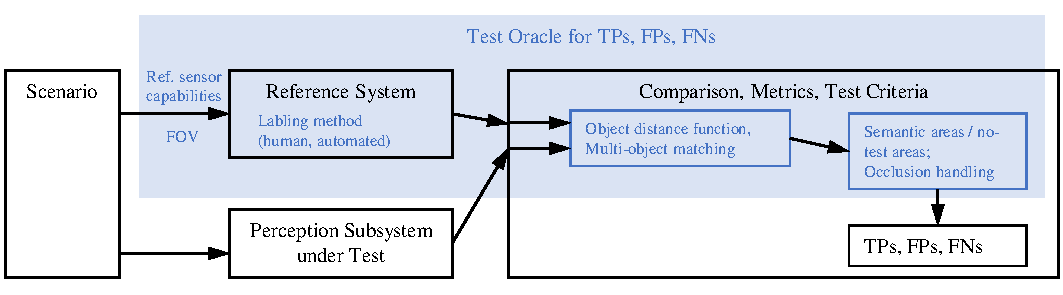
\includegraphics[width=\textwidth]{img/taxonomy_with_oracle.pdf}
	
	\caption{Test oracle for identifying TPs, FPs, and FNs, mapped into the taxonomy for ADS perception testing \cite{Hoss2022review, stellet2015testing}. Implemented test oracles can differ from this exemplary illustration. For example, certain aspects can be located either under ``Reference System" or ``Comparison, Metrics, Test Criteria".
		% TODO: insert subsection numbers.
	}
	\label{fig:oracle_in_taxonomy}
\end{figure*}


\subsection{Definition of terms \& abbreviations}
Unless stated otherwise, the following term definitions and acronyms hold throughout this paper.

\subsubsection{Object} \label{def:object}
From ISO 23150:2021 \cite{ISO_23150_2021_data_communication}: 
``representation of a real-world entity with defined boundaries and characteristics in the vehicle coordinate system".
This paper narrows down this definition to Layer 4 of the 6-layer-model \cite{Scholtes20216lmAccess}. An object can span over one or multiple time steps. 

\subsubsection{Object under Test (OuT)} \label{def:out} Perception subsystem of a driving automation system. It comprises both hardware and software and it outputs an object list in each time step. Note: The ``object" in OuT must not be confused with the more general \textit{object} defined above (Sec. \ref{def:object}).

\subsubsection{True Positive (TP)} \label{def:tp} The circumstance that an object in the data under test matches with an object in the reference data (Fig. \ref{fig:top_down_all}, 1).

\subsubsection{False Positive (FP)} \label{def:fp} The circumstance that an object in the data under test does not match with any object in the reference data (Fig. \ref{fig:top_down_all}, 2). 

\subsubsection{False Negative (FN)} \label{def:fn} The circumstance that no object in the data under test matches with a given object in the reference data (Fig. \ref{fig:top_down_all}, 3).

\subsubsection{True Negative (TN)} \label{def:tn} The circumstance that the non-existence of an object in the data under test matches with the non-existence of an object in the reference data. Since world modeling in form of object lists represents the non-existence of objects only implicitly, TNs are not quantifiable in the context of this paper.

%\subsubsection{Matching method} \label{def:matching_method} Those parts of the test method that influence the identification of TPs, FPs, and FNs. 
% based on an object list under test and a reference object list. 

% OMG I finally got the difference between method and methodology!! I should use method much more often now. But sometimes, methodology is the term to use (when I analyze different methods).

\subsubsection{Matching result} \label{def:matching_result} General term or category of the mutually exclusive circumstances TP, FP, FN.  


%\subsubsection{Matching} As part of a test method, identifying TPs, FPs, and FNs based on the object lists of OuT and reference system. 

\subsubsection{Object association} \label{def:association} As part of a perception algorithm, deciding which existing object track a novel object detection belongs to. Not to be confused with \textit{matching}, which is a concept of the test method (adopted from \cite{Luiten2020hota}).

\subsubsection{(Test) oracle} \label{def:oracle} 
%The mechanism that determines whether a test passes or fails (see also survey by Barr et al. \cite{Barr2015oracle}).
In the present paper, \textit{(test) oracle} refers to the mechanism that identifies TPs, FPs, and FNs, where the test scenario and the OuT are given (Fig. \ref{fig:oracle_in_taxonomy}).

\subsubsection{Reference System (ReS)}
\label{def:reference_system}
Perception system that observes the scenario and whose outputted object list serves as a desired reference for the object list under test. 

% oracle problem in \cite{Zhang2022ml_testing}


\section{Methods}
\label{sec:method}

% We define the criteria for identifying TP, FP, and FN in the following way.

When human experts observe a top-down view representation of a traffic scene with an overlaid object list under test (Fig. \ref{fig:top_down_all}), they can typically make the following statements:
\begin{itemize}
	\item the ADS \textit{did} see the other road user
	\item the ADS \textit{did not} see the other road user 
	\item the ADS saw a road user \textit{that did not exist}.
\end{itemize}

We currently assume that an ideal test oracle exactly reproduces such human expert statements when it identifies TPs, FNs, and FPs correspondingly.
A human reference for the definition of a test oracle is beneficial for the human comprehensibility of the overall safety argumentation. 
However, for the sake of comparability of test results, the actual oracle should ideally be exactly reproducible and therefore contain as little human intuition as possible. 

Consequently, we aim at encoding our human intuition for a test oracle into unambiguous criteria. 
Our method to do this primarily consists of noting down and structuring all aspects that we consider relevant based on our previous experience. 
This experience consists of object-level online data fusion, object-level perception error modeling, testing of object perception against aerial reference data, and scenario elicitation from traffic recordings for safety assurance. 


As we apply this experience-based oracle definition to a popular perception challenge (Sec. \ref{sec:perception_challenge}), we refine it and demonstrate its practical applicability. 


%oracle is also at least partially based on intuition that is naturally impossible to specify explicitly. 
%Therefore, we intend to define criteria that allow to specify this human intuition as close as possible. 


%Eliminating the uncertainty of human intuition from the test oracle might make it more rigorous and formal, but for the time being, we justify our human reference for the test oracle as follows. 
%Since the safety argumentation is performed and evaluated by humans, its claims and evidences should be 


%\footnote{Eliminating informal human intuition from the oracle for TPs, FPs, and FNs could be beneficial, but this topic is outside the scope of this paper.}. 
%This assumption can be justified by the fact that human judges 


% Our goal is to list all relevant aspects of the test method 

%While other works use machine learning in the test method to reproduce these human observations \cite{Florbaeck2016.matching.offline, Sondell2018}, our goal is to make the features, criteria, and thresholds of the oracle as explicit as possible.



  



% Experience. No special method. 



\section{Defining a test oracle for TPs, FPs, FNs}
\label{sec:criteria}



\begin{figure*}[t]
	\centering
	\vspace*{2mm}
	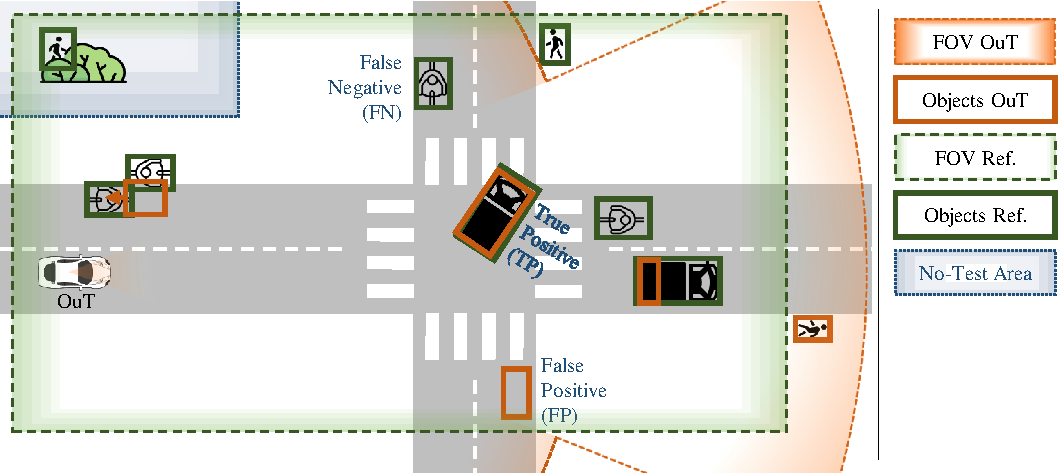
\includegraphics[width=\textwidth]{img/top_down_fitting_slide.pdf}
	
	\caption{ While objects A-C appear obvious, the desired identification of TPs, FPs, and FNs from objects D-L requires a purposefully defined test oracle. 
		%A clear definition of the test oracle is needed to understand how it identifies TPs, FPs, and FNs from the given objects A-L. 
		%Aspects of road traffic and geometry that the test oracle covers.
	}
	\label{fig:top_down_all}
\end{figure*}


A test oracle that identifies TPs, FPs, and FNs is a logical part of a testing activity (Fig. \ref{fig:oracle_in_taxonomy}), it deals with spatial relations in a traffic scene (Fig. \ref{fig:top_down_all}), and with temporal aspects of object matching (Fig. \ref{fig:timeline}).

This section details the aspects illustrated in the mentioned figures in natural language. 
% We intentionally avoid a more formal, more technical, or more specific description in order to keep it generally applicable to as many test oracles as possible without prescribing an internal structure and without . 
% DO THIS WHY NATURAL LANGUAGE HERE IN THE DISCUSSION!
It first treats the simple case of deterministic object representations in a single time frame (Sec. \ref{sec:oracle_simple}) and then covers temporal aspects (Sec. \ref{sec:oracle_time}) and probabilistic object descriptions (\ref{sec:oracle_probabilistic}).
The actual aspects that collectively define the workings of the test oracle are given one level deeper (e.g. Sec. \ref{sec:fov_ref}). 

In this whole section, we assume that any FP or FN is an undesired penalty to the OuT. 

%In general: matching of tracks under test to reference tracks. This boils down to:

\subsection{Matching deterministic objects in a single time frame}
\label{sec:oracle_simple}

In this subsection, we assume that the object lists of OuT and ReS are perfectly temporally synchronized. 

\subsubsection{Perspective and field of view of reference data}
\label{sec:fov_ref}
In general, the fields of view (FoV) can differ between OuT and ReS. This can lead to undesired FNs and FPs in areas where only one of both FoVs is present. 
In Fig. \ref{fig:top_down_all}, the OuT has no chance to detect the pedestrian E, given its FoV. 
Likewise, the ReS has no chance to detect the pedestrians K and J, given its FoV. 

Differing FoVs can originate from different perspectives, different sensor choices, and different data processing methods.
First, the perspective of a camera-equipped drone results in a rectangular FoV, whereas the OuT's FoV on the ground typically consists of circles and circular sectors (Fig. \ref{fig:top_down_all}).
Second, reference data could be labeled only on the OuT's cameras and lidars, whereas the OuT additionally uses a radar whose range exceeds the other sensors. 
Third, the OuT's detection algorithm might propose object hypotheses on distant raw data where the ReS refuses to label objects.

Whether or not the OuT should be penalized for missing pedestrian E in Fig. \ref{fig:top_down_all} depends on the test objective. 
If only the perception algorithm is tested, then overlapping areas of the ReS could be trimmed to enable a fair evaluation.
However, if the FoV of the OuT is put under test, too, and it is supposed to cover the entire ReS's FoV, then the ReS's FoV should not be trimmed and the FN E should be identified. 

In summary, a clear definition of the ReS's FoV relative to the OuT's FoV is crucial for a clearly defined test oracle. 

\subsubsection{Reference system hardware}
\label{sec:ref_hw}

The way in which the ReS hardware differs from the OuT hardware influences the test oracle. 
In the simplest case, ReS and OuT share the very same sensor hardware and just differ in their data processing. 
This case would exclude unexpected FPs and FNs based on hardware differences, which is desired if only the OuT's data processing is focused. 

If, however, also the OuT's hardware is focused, then the ReS should contain sensors with superior properties. 
For example, if ReS and OuT consist of different sensor modalities, then in adverse weather conditions, the ReS could detect objects that the OuT cannot detect (FNs). 
%Depending on what part or parts of the OuT is focused in the testing activity (hardware/data processing), these FNs can be desired or undesired.



\subsubsection{Reference system labeling and data processing}
\label{sec:ref_processing}

In general, the extraction of an object list from the raw reference data can consist of programmed software, machine-learned modules, and human interaction. 

Specified labeling policies fall under this category. They include details such as how objects are classified, criteria for including and omitting objects, which parts of objects shall be inside or outside their bounding boxes, how to label in case of partial or full occlusions and much more.
The labeling policy and their realization influence the reference data quality, which, in turn, influences the test oracle. 
%For example, labeling can be fully automated, semi-automated, or manual, where each way impacts the labeling quality in a different way. 

This aspect of the test oracle can be characterized by its internal workings and its outputted results. 
The internal workings include the programmed modifications that the data undergo, the capabilities of the machine-learned modifications, and the relevant human aspects (when and how do humans interact with the data).
The outputted results, namely, the reference object list, can be described by statements or statistics about accuracy and precision of the labels. 
A higher-level reference system or procedure could be needed for this purpose.


\subsubsection{Semantic areas and no-test areas}
\label{sec:semantic_areas}
semantic areas in the road infrastructure that tell where to test

\subsubsection{Object distance function in state space}
\label{sec:distance_function}
including penalties (object classifications?) and thresholds. 
Can be a mathematical metric or not. 

\subsubsection{Multi-object matching algorithm}
\label{sec:multi_object_matching}
Not only 1:1, but also n:n, as e.g. Brahmi \cite[Sec. 10.3]{Brahmi2020diss} describes it. E.g. hungarian or auction. 


\subsubsection{Geometrical alignment of OuT and ReS}
How are both object lists put into the same coordinate system, which is necessary for a subsequent comparison?

Ideally, the coordinate transformation's inaccuracy and imprecision are negligible. 
However, errors in the geometrical alignment can affect the test oracle. 
E.g. sensor mounting positions not correctly calibrated. 
E.g. transformation from top-down view (e.g. moving UAV or infrastructure sensor) to vehicle coordinate system imprecise. 


%\begin{enumerate}
%\item object distance functions in state space, including penalties and thresholds
%\item multi-object association algorithms. Not only 1:1, but also n:n, as e.g. Brahmi \cite[Sec. 10.3]{Brahmi2020diss} describes it.
%\item reference data and labeling characteristics
%\item fields of view of reference data relative to OuT  (FOV of OuT does not belong to the test oracle)
%\item semantic areas in the road infrastructure that tell where to test
%\end{enumerate}

\subsection{Generalization to object tracks over time}
\label{sec:oracle_time}

Brahmi \cite{Brahmi2020diss} did quite some stuff on timing.


\begin{figure}[t]
	\centering
	\vspace*{2mm}
	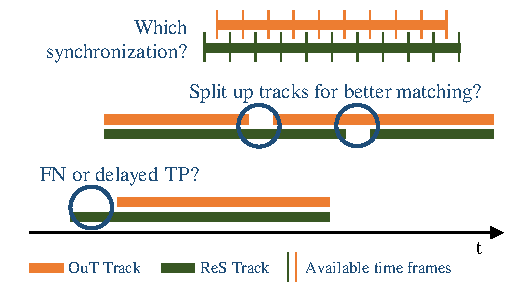
\includegraphics[width=0.49\textwidth]{img/timeline.pdf}
	\caption{Temporal aspects of the test oracle. TODO: synchronization/interpolation?
	}
	\label{fig:timeline}
\end{figure}

\subsubsection{Level of object lists}

When time is also considered, the level of the evaluated object lists becomes important:
\begin{itemize}
\item detections
\item tracks
\item single frames from tracks
\item tracklets
\end{itemize}



\subsubsection{Association of tracks}


\subsubsection{Temporally incomplete tracks}
\label{sec:temp_incomplete}

\subsubsection{Treatment of latency and delays}
\label{sec:temp_latency}

\subsubsection{Synchronization of measurement time stamps}
\label{sec:temp_sync}

Synchronization between OuT and reference system (same measurement frequency). 
Also interpolation and extrapolation.

Aligning time stamps for arbitrary asynchronous measurement frequencies. Brahmi \cite[Sec. 10.2.7]{Brahmi2020diss} interpolates the reference data time stamps onto the OuT time stamps.


%\begin{enumerate}
%\item Brahmi \cite{Brahmi2020diss} did quite some stuff on timing
%\item temporally incomplete tracks 
%\item latency of the OuT
%\item synchronization between OuT and reference system (same measurement frequency)
%\item aligning time stamps for arbitrary asynchronous measurement frequencies. Brahmi \cite[Sec. 10.2.7]{Brahmi2020diss} interpolates the reference data time stamps onto the OuT time stamps.
%\end{enumerate}


\subsection{Generalization to probabilistic object descriptions}
\label{sec:oracle_probabilistic}

\subsubsection{Probabilistic FoVs}
What if no clear FoV border exists?

\subsubsection{Probabilistic thresholding}
\label{sec:prob_thresholding}
if we choose hard threshold values to avoid association of certain 


%\begin{enumerate}
%\item if we choose hard threshold values to avoid association of certain 
%\end{enumerate}


\section{Example Case Studies}

Or outsource them to the next paper?

Use as much mathematical notation as possible here! (Really?)

\subsection{Submission at Perception Challenge}
\label{sec:perception_challenge}

Describe an example submission at the leaderboard of Waymo Open Dataset. 

Labeling specifications\footnote{\url{https://github.com/waymo-research/waymo-open-dataset/blob/master/docs/labeling_specifications.md}}.

Description of perception challenge\footnote{\url{https://waymo.com/open/data/perception/}}


\subsection{External Reference System}

Use inD data with a simulated ego vehicle and simulated data under test.
Use the Lanelet2 map (converted to the omega format) to include and exclude certain areas.

\begin{table*}[t]
	\centering
	\caption{Test oracles expressed in the terminology of this paper}
	\label{table:case_study}
	\begin{tabularx}{\linewidth}{
			>{\hsize=0.40\hsize}X 
			>{\hsize=0.8\hsize}X 
			>{\hsize=0.8\hsize}X 
		} 
		\toprule
		\textbf{Criterion} & \textbf{Waymo Challenge} & \textbf{Drone Testing} \\
		\midrule
		Simple aspects %
		& stuff
		& stuff \\
		\hline
		Temporal aspects 
		& stuff
		& stuff  \\ 
		\hline
		Probabilistic aspects 
		& stuff
		& stuff  \\ 
		\bottomrule
	\end{tabularx}
\end{table*}


\subsection{How do TP statistics change when the oracle criteria vary?}

I could include such a case study on simulated data. The omega format with the perception testing dashboard would be handy for that.


\section{Discussion of Research Questions}
\label{sec:discussion}

We have presented a generic set of relevant conditions for specifying a test oracle that identifies TP, FP, and FN. 
However, even this set of conditions might not be generic enough to specify all possible concepts of such a test oracle. 


\subsubsection{Awareness of Symbol Grounding Problem}

TODO

Just like it is hard to define what e.g. a pedestrian is, it is also hard to define what a true positive is. 
Humans that use these terms in their natural language have learned their meanings over time, but are often not fully aware of the exact criteria that define a pedestrian or a true positive, for example.  

Humans tend to say ``the ADS did not see the pedestrian". While for some world model instances, such a statement is obvious, for other world model instances, it is highly complex to unambiguously define what it means that one road user sees another one. 


\subsubsection{Design of Future Safety-Oriented Perception Metrics}

Metrics that rely on a distinction between, TPs, FPs, FNs have these difficulties. 

In contrast, Task-Oriented Metrics that employ a downstream driving function or assumptions thereof don't manually feature-engineer the criteria for must-see objects, but have that additional complexity. 


\subsection{Compliance with standards}

TODO

Some standards, e.g. UL4600 \cite[Sec. 8.4.1.2]{UL4600_voting_2019} suggest providing statistics of FPs and FNs. 
Since a safety argumentation to comply with a standard should contain the least possible ambiguity, this paper aims at providing guidance to define FPs and FNs as clearly as possible. 



\subsection{More formal definition of test oracle}

It is hard because some things are hard to formalize.
A modular technical description of a test oracle would already partially predetermine the arrangement of its modules, or the internal structure of the test oracle. This, however, can be flexible. For example, certain objects or semantic areas could be ignored at the very beginning of the testing activity, or at the very end. 
Future work how far a formal description can go without unnecessarily prescribing internals of the test oracle. 



\section{Related Work}
\label{sec:related_work}

Only related work here that is about the definition of TPs, FPs, and FNs. 
All further relevant literature sources that do not explicitly focus on defining TPs will be referenced as they become relevant in other sections. 

Florbäck et al. \cite{Florbaeck2016.matching.offline} and Sondell and Svensson \cite{Sondell2018} investigate how machine learning can reproduce human associations of objects under test to reference objects.


\section{Conclusion}
\label{sec:conclusion}

Future work includes a more formal description of a test oracle, potentially by means of a domain-specific language.



%\section{Introduction}
\label{sec:introduction}

Will refer to \cite{Hoss2022review}.

% \section{Related Work}
\label{sec:related_work}

% \section{Method}
\label{sec:method}

Describe your experimental design with enough detail so that a competent colleague could reproduce your results. Passive voice sometimes functions well in the Methods section.
Elsewhere in a scientific paper, however, it should rarely be chosen. 

\begin{figure}
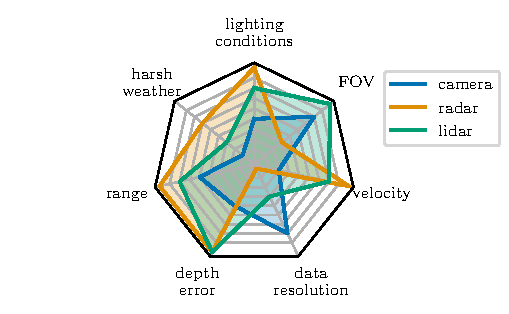
\includegraphics{img/spider_sensorcomp.pdf}
\centering
\caption{Figures MUST be in PDF (everything that can be a vector must be a vector) or PNG format to prevent issues with the arXiv upload.}
\label{fig:compare_sensors}
\end{figure}

% \section{Evaluation}
\label{sec:evaluation}


% \section{Conclusion}
\label{sec:conclusion}

Discussion and Outlook
% \section{Acknowledgment}
\label{sec:acknowledgment}

This work results partly from the KIGLIS project supported by the German Federal Ministry of Education and Research (BMBF), grant number 16KIS1231.

% -------------------------- REFERENCES -------------------------------

{\small
\bibliographystyle{IEEEtran}
\bibliography{literature/AllSourcesMHO.bib}
}

\end{document}
